\documentclass[a4paper,10pt]{report}
\usepackage{graphicx}


\begin{document}
\section*{Influence of the topology of cultural networks  on the equilibrium of an exchange-based economy}

The study of past societies can help researchers to understand long-term dynamics of social interaction. Within this context, the Roman Empire shows  interesting properties that could feed current debates on economy, such as the relation between resilience and degree of interconnectivity, or the relevance of institutions in phases of crisis. It seems relevant to understand an economy that lasted over 400 years. Nonetheless, doing so is a challenging task. Traces of the economic activity in the archaeological record are scarce and heterogeneous. They only explain fragments of the entire economy and they only do this for a particular moment in time and space.

Computational tools such as computer simulation, coupled with complexity theory, can help us to face these challenges. They provide a set of methods and theories to analyse and test the hypotheses we can make about the Roman economy. Even with a partial knowledge of the mechanisms but with simple hypothesis, we can simulate and analyse the dynamics of the whole system, compare it to the available data and quantify the plausibility of the hypothesis and theories used.

In the particular case of the economy, we are interested on exploring a system based on these main components: (i) the interaction between the actors of the system, (ii) the evolution of such interaction and (iii) the resulting global dynamics. In other terms, we see the Economy as a cultural process evolving through time and where interaction between individuals is central. Thus, we think that network analysis and methods from cultural evolution studies are the best suited tools provided by complex systems and computer simulation to tackle the problem. 


We think that the structural properties of the networks that allow the agents to exchange knowledge, goods and believes, are crucial for the development and maintenance of the economy, moreover in a society such as Rome where we expect that the communication system limits the rate of exchange (both of good and information) over distance. Here, we specifically assess the question of how the communication network, the one that allow individuals to know and learn the behavior of the others (what we call the local cultural environment), could influence the global dynamics of the whole society’s economy. More precisely, we want to detect and quantify the different cultural conditions that lead to the emergence of an optimal and stable decentralized free market (as it is the case in the figure 1).


\begin{figure}[h!]
	\center
	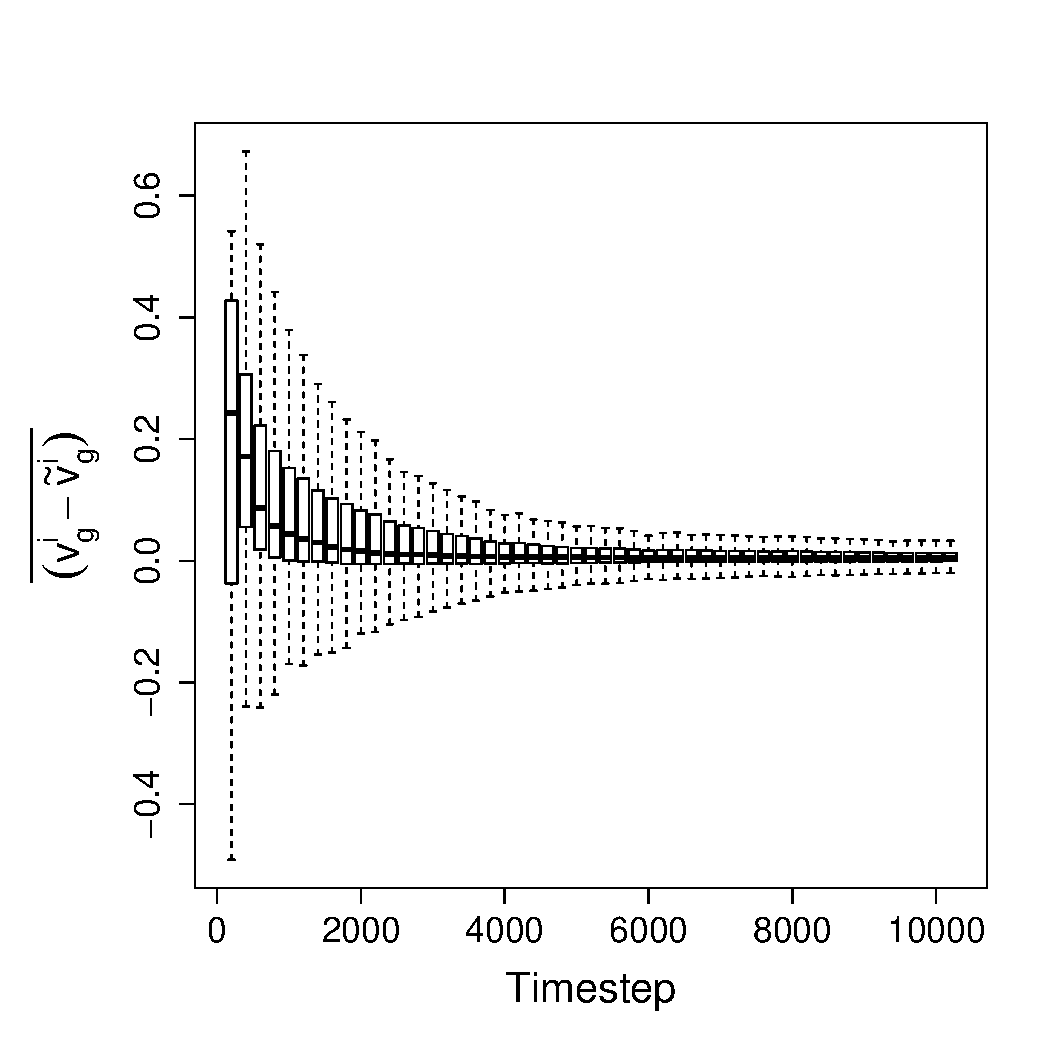
\includegraphics[width=8cm]{img/ClearingPriceDistanceEvolutionForTrade-G3N500.pdf}
\caption{This figure shows the convergence of the value attributed by the agent to the goods of the system toward the optimal value of the goods. In this experiment we test the extreme case where all individuals are fully connected to all other individuals. The optimal values are the values that allow everybody to sell and buy every goods in the system in the optimal quantities.}
\end{figure}

To do so, we use an exchange-based economy model, where individuals produce a good that must be traded in order to get the other goods they need. The agents belong to a cultural environment i.e. a local interaction network that enables them to know their neighbors' trading strategies. In this manner, they take part in a payoff-biased, social learning process whereby they can change their own strategy by imitating the most successful individuals.

The first use of this model has shown to converge to an optimal market without a central authority. The local interactions  were not restricted in any sense: all agents were able to know the economic success  of all the others and imitate whoever they choose. This resulted in the totality of the agents being able to exchange their goods and achieving their goals without central coordination, and thus converging to an optimal and stable state as a system.

In the current work we want to study to what extent this convergence capacity depends on the cultural networks of the individuals. To do so, we compare three types of network topologies, namely, random, small-world and scale-free networks. Each topology represents different conditions of cultural interactions. For each case, we run simulations and measure the properties of the resulting economic dynamics. We aim to quantify under which particular trade and cultural conditions a stable, decentralized and optimal economy is able to emerge.

This theory-building approach will enhance our understanding of the relevance of cultural change in past trade networks. The exercise will allow us to generate hypotheses that ultimately can be evaluated against archaeological evidence.
\end{document}

%%================================================================
%
%The study of past societies can help researchers to understand long-term dynamics of social interaction. Within this context, the Roman Empire shows some properties that seem particularly relevant to current debates on economy such as the relation between resilience and degree of interconnectivity, or the relevance of institutions in phases of crisis. In this context, it seems relevant to understand an economy that lasted over 400 years.
%Understanding the mechanism behind the Roman economy is an important goal. It wouldwill help to solve the old historical debate on the nature of the roman market as well as allow to better understand our own economic system. Nonetheless doing so is a challenging task.Traces of the economic activity in the archaeological record are scarce and heterogeneous, and the rare reliable historical sources give us only clues on small parts of the whole problem. They only explain fragments of the entire economy, and they only do this for a particular moment in time and space.
%
%Computer simulation, coupled with complex systems approach, allow the researchers to address such issues. Computational tools such as computer simulation coupled with complexity theory can help us to face these challenges. They provide a set of tools and theories to analyse and test the hypotheses we can make about the roman economy. Even with a partial knowledge of the mechanism but with simple hypothesis, we can simulate and analyse the dynamics of the whole system, compare it to the available data and quantify the plausibility accuracy of the hypothesis and theories used.
%
%In the particular case of the economy, we are interested on exploring a system based on these main components: (i)...
%In the particular case of the economy, we think that the central mechanisms are (i) the interaction between the actors of the system, (ii) the evolution of such interaction and (iii) the resulting global dynamics. In this perspective we think that network analysis and methods from cultural evolution studies are the best suited tools provided by complex systems and computer simulation to tackle the problem.
%
%In this study, we specifically assess the question on how the local cultural environment of the individuals in a society could influence the global dynamics of its economy. More precisely we want to detect and quantify the different cultural conditions that lead to the emergence of an optimal and stable decentralized free market.
%
%To do so, we use a trade model in which individuals produce a good that must be exchanged in order to get the other goods they need. The agents belong to a cultural environment i.e. a local interaction network that enables them to know their neighbors' trading strategies. The agents can then change their own strategy by imitating the most successful individuals.
%
%The first use of this model has shown to converge to an optimal market without a central authority. The local interactions  were not restricted in any sense: all agents were able to know the economic success  of all the others and imitate whoever they choose. This resulted in the totality of the agents being able to exchange their goods and achieving their goals without central coordination, and thus converging to an optimal and stable state as a system.
%
%In the current work we want to study to what extent this convergence capacity depends on the cultural networks of the individuals. To do so, we compare three types of network topologies, namely, random, small-world and scale-free networks. Each topology represents different conditions of cultural interactions. For each case, we run simulations and measure the properties of the resulting economic dynamics. We aim to quantify under which particular trade and cultural conditions a stable, decentralized and optimal economy is able to emerge.
%
%In following works we will confront those result against the Archaeological and Historical evidence in order to evaluate which of the previously studied case could be more appropriate to describe the Roman Economy.
%
%
%This theory-building approach will enhance our understanding of the relevance of cultural change in past trade networks. The exercise will allow us to generate hypotheses that ultimately can be evaluated against archaeological evidence.
%
%
%
